%%%%%%  CRONOLOGIA ABCS  %%%%%%
\chapter{Cronología de publicaciones sobre sistemas ABC}\label{apendix:ApendiceCronologiaABC}

Sistemas \GLS{ABC} que usan biometría palmar como rasgo identificativo en su sistema biométrico.

\cite{nanavati2011biometric}.

\begin{landscape}
 \begin{figure}
  \centering
  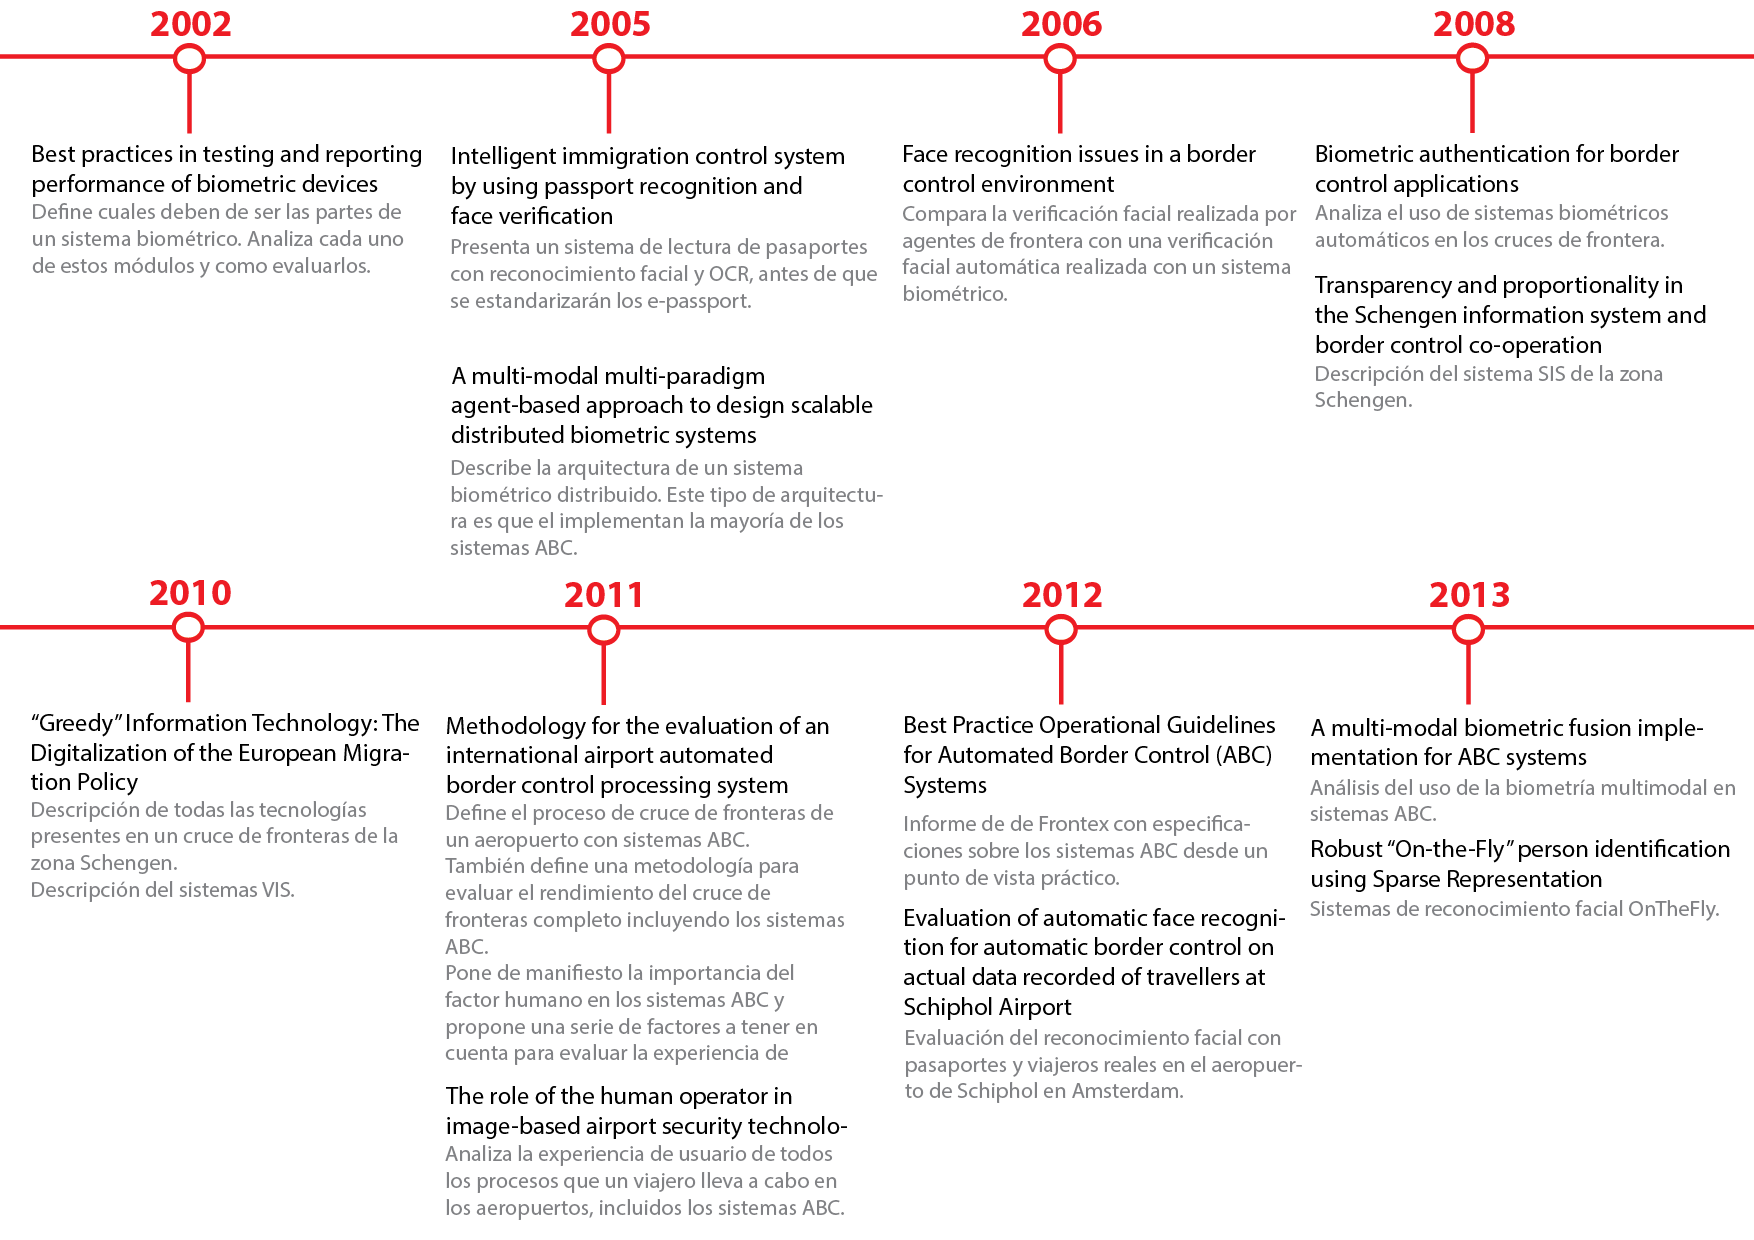
\includegraphics[width=1.4\textwidth]{ch-sistemasABC/images/ch-ImagenesApendices/00_CRONOLOGIA_ABC.png}
  \label{fig:00_CRONOLOGIA_ABC}
 \end{figure}
\end{landscape}

\begin{landscape}
 \begin{figure}
  \centering
  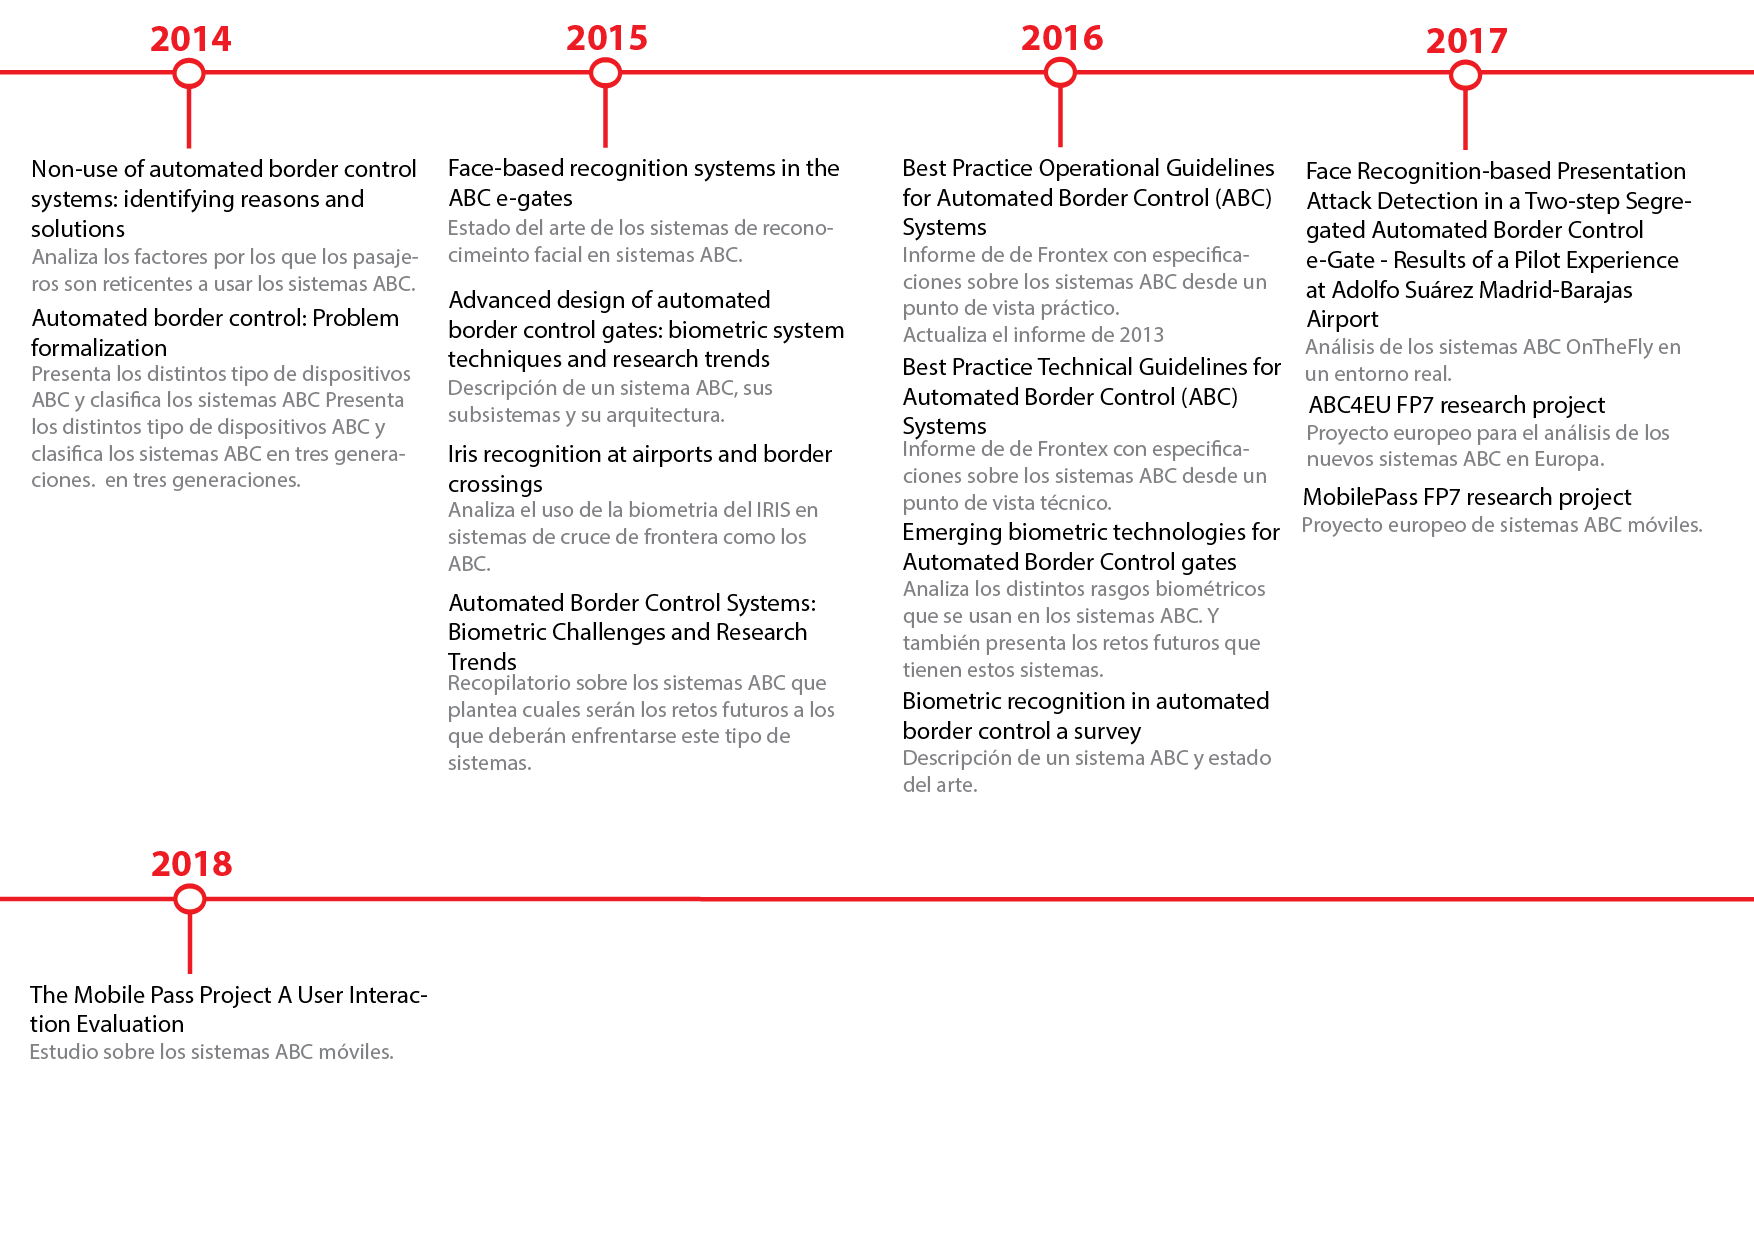
\includegraphics[width=1.4\textwidth]{ch-sistemasABC/images/ch-ImagenesApendices/01_CRONOLOGIA_ABC.png}
  \label{fig:01_CRONOLOGIA_ABC}
 \end{figure}
\end{landscape}

% $\textbf{2002}$

% \cite{mansfield2002best}
% Define cuales deben de ser las partes de un sistema biométrico. Analiza cada uno de estos módulos y como evaluarlos.

% $\textbf{2005}$

% \cite{kim2005intelligent}
% Presenta un sistema de lectura de pasaportes con reconocimiento facial y \GLS{OCR}, antes de que se estandarizarán los \gls{e-passport}.

% \cite{gamassi2005multi}
% Describe la arquitectura de un sistema biométrico distribuido. Este tipo de arquitectura es que el implementan la mayoría de los sistemas \GLS{ABC}.

% $\textbf{2006}$

% \cite{kosmerlj2006face}
% Compara la verificación facial realizada por agentes de frontera con una verificación facial automática realizada con un sistema biométrico.

% $\textbf{2008}$

% \cite{kwon2008biometric}
% Analiza el uso de sistemas biométricos automáticos en los cruces de frontera.

% \cite{karanja2008transparency}
% Descripción del sistema \GLS{SIS} de la zona \Gls{Schengen}.

% $\textbf{2010}$
% \cite{brom2010greedy}
% Descripción de todas las tecnologías presentes en un cruce de fronteras de la zona \Gls{Schengen}. 

% Descripción del sistemas \GLS{VIS}.

% $\textbf{2011}$
% \cite{macleod2011methodology}
% Define el proceso de cruce de fronteras de un aeropuerto con sistemas \GLS{ABC}.

% También define una metodología para evaluar el rendimiento del cruce de fronteras completo incluyendo los sistemas \GLS{ABC}

% Pone de manifiesto la importancia del factor humano en los sistemas \GLS{ABC} y propone una serie de factores a tener en cuenta para evaluar la experiencia de usuario de los sistemas \GLS{ABC}. 

% \cite{graves2011role}
% Analiza la experiencia de usuario de todos los procesos que un viajero lleva a cabo en los aeropuertos, incluidos los sistemas \GLS{ABC}.

% $\textbf{2012}$

% \cite{FRONTEX2012OpeReport}
% Informe de de \Gls{frontex} \cite{FRONTEXOnLine} con especificaciones sobre los sistemas \GLS{ABC} desde un punto de vista práctico.

% \cite{spreeuwers2012evaluation}
% Evaluación del reconocimiento facial con pasaportes y viajeros reales en el aeropuerto de Schiphol en Amsterdam. 

% $\textbf{2013}$

% \cite{cantarero2013multi}
% Análisis del uso de la biometría multimodal en sistemas \GLS{ABC}. 

% \cite{raghavendra2013robust}
% Sistemas de reconocimiento facial \textit{OnTheFly}.

% $\textbf{2014}$

% \cite{oostveen2014non}
% Analiza los factores por los que los pasajeros son reticentes a usar los sistemas \GLS{ABC}.

% \cite{gorodnichy2014automated}
% Presenta los distintos tipo de dispositivos \GLS{ABC} y clasifica los sistemas \GLS{ABC} en tres generaciones.  

% $\textbf{2015}$

% \cite{del2015face}
% Estado del arte de los sistemas \GLS{ABC}.

% \cite{labati2015advanced}
% Descripción de un sistema \GLS{ABC}, sus subsistemas y su arquitectura.

% \cite{daugman2015iris}
% Analiza el uso de la \gls{biometria} del IRIS en sistemas de cruce de frontera como los \GLS{ABC}.

% \cite{labati2015automated}
% Recopilatorio sobre los sistemas \GLS{ABC} que plantea cuales serán los retos futuros a los que deberán enfrentarse este tipo de sistemas.

% $\textbf{2016}$

% \cite{FRONTEX2016OpeReport}
% Informe de de \Gls{frontex} \cite{FRONTEXOnLine} con especificaciones sobre los sistemas \GLS{ABC} desde un punto de vista práctico.

% Actualiza el informe de $2013$ \cite{FRONTEX2012OpeReport}.

% \cite{donida2016emerging}
% Analiza los distintos rasgos biométricos que se usan en los sistemas \GLS{ABC}. Y también presenta los retos futuros que tienen estos sistemas. 

% \cite{FRONTEX2016TechReport}
% Informe de de \Gls{frontex} \cite{FRONTEXOnLine} con especificaciones sobre los sistemas \GLS{ABC} desde un punto de vista técnico.

% \cite{labati2016biometric}
% Descripción de un sistema \GLS{ABC}.

% $\textbf{2017}$

% \cite{del2017face}
% Análisis de los sistemas \GLS{ABC} \text{OnTheFly} en un entorno real. 

% \cite{ABC4EUOnline}
% Proyecto europeo para el análisis de los nuevos sistemas \GLS{ABC} en Europa.

% \cite{MobilePassOnline}
% Proyecto europeo de sistemas \GLS{ABC} móviles. 

% $\textbf{2018}$

% \cite{blanco2018mobile}
% Estudio sobre los sistemas \GLS{ABC} móviles.

%%%%%%  CRONOLOGIA BIOMETRIA  %%%%%%
\chapter{Cronología de publicaciones sobre biometría}\label{apendix:ApendiceCronologiaBiometria}

\begin{landscape}
 \begin{figure}
  \centering
  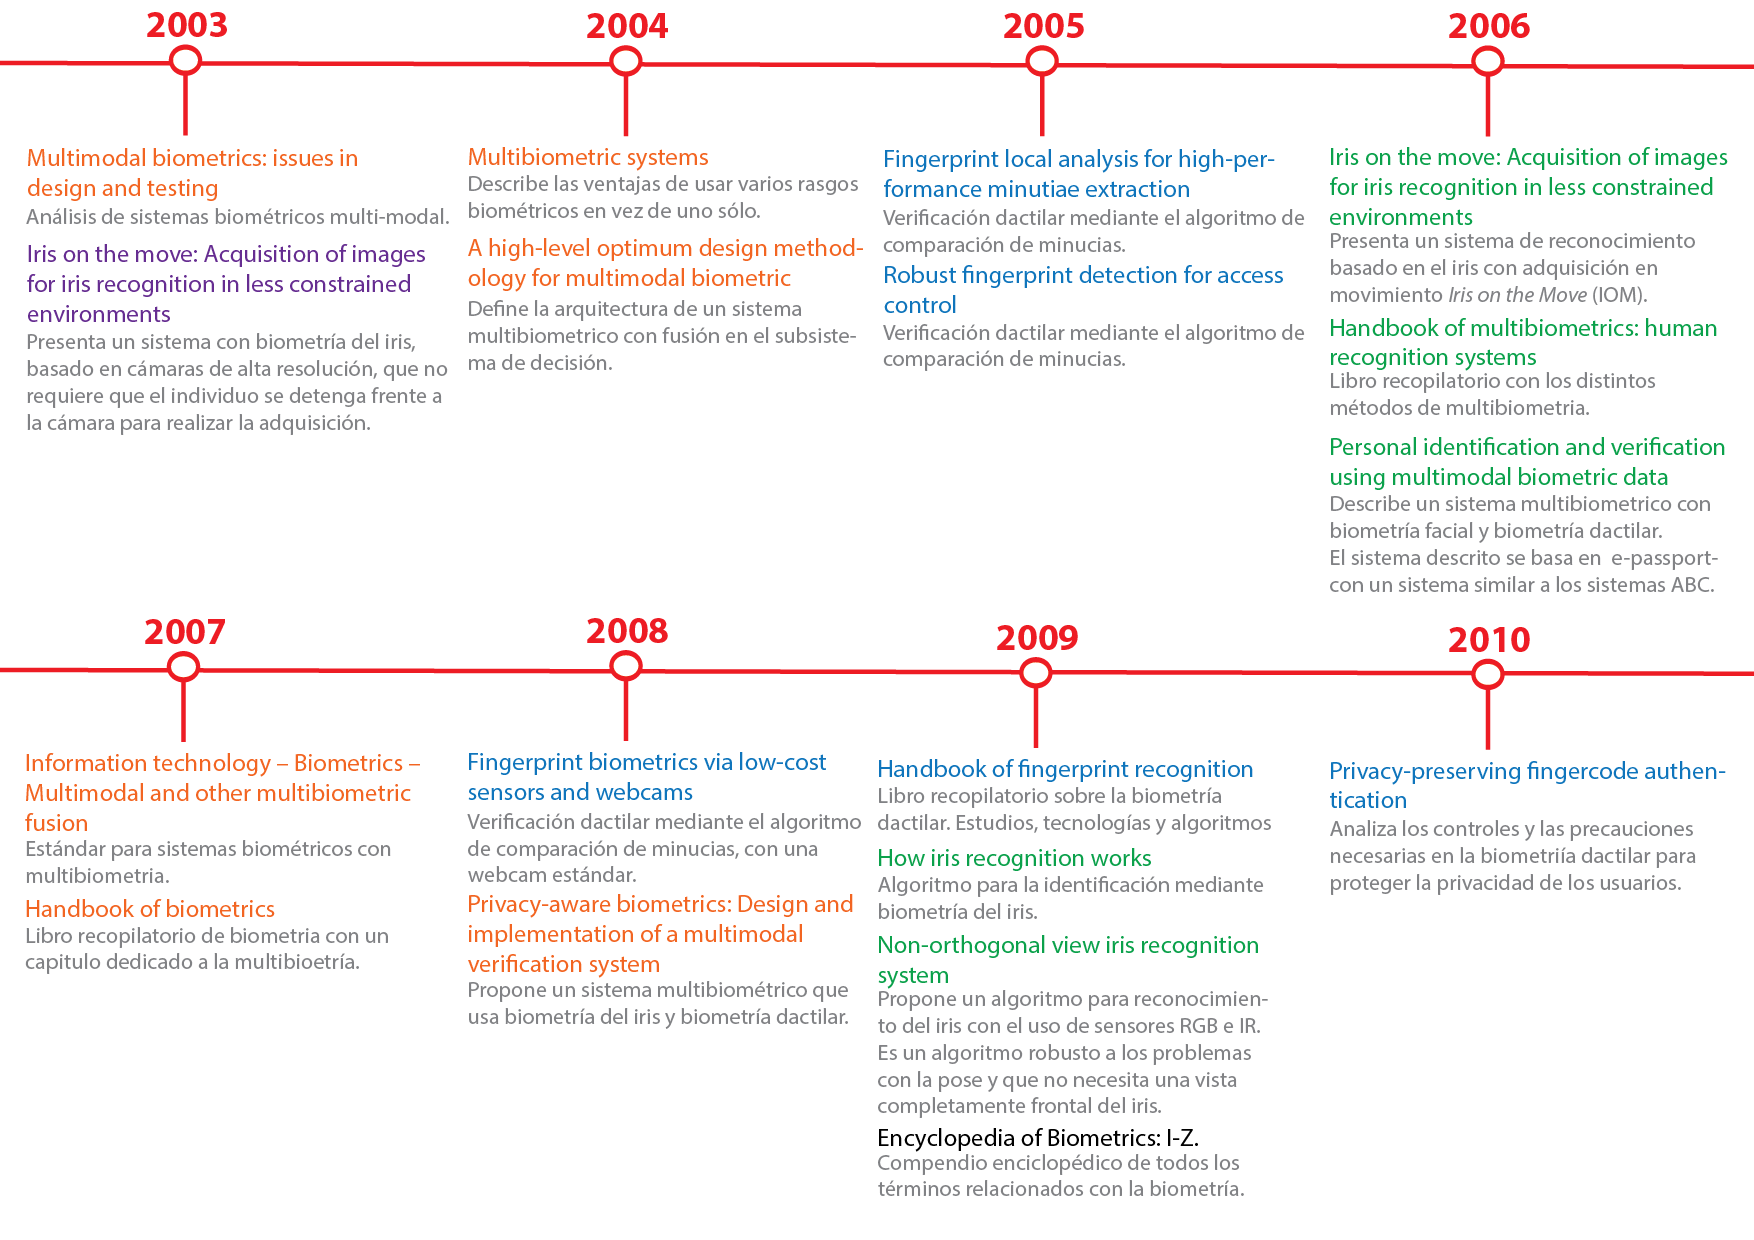
\includegraphics[width=1.4\textwidth]{ch-sistemasABC/images/ch-ImagenesApendices/CRONOLOGIA_BIOMETRIA-01.png}
  \label{fig:00_CRONOLOGIA_BIOMETRIA}
 \end{figure}
\end{landscape}

\begin{landscape}
 \begin{figure}
  \centering
  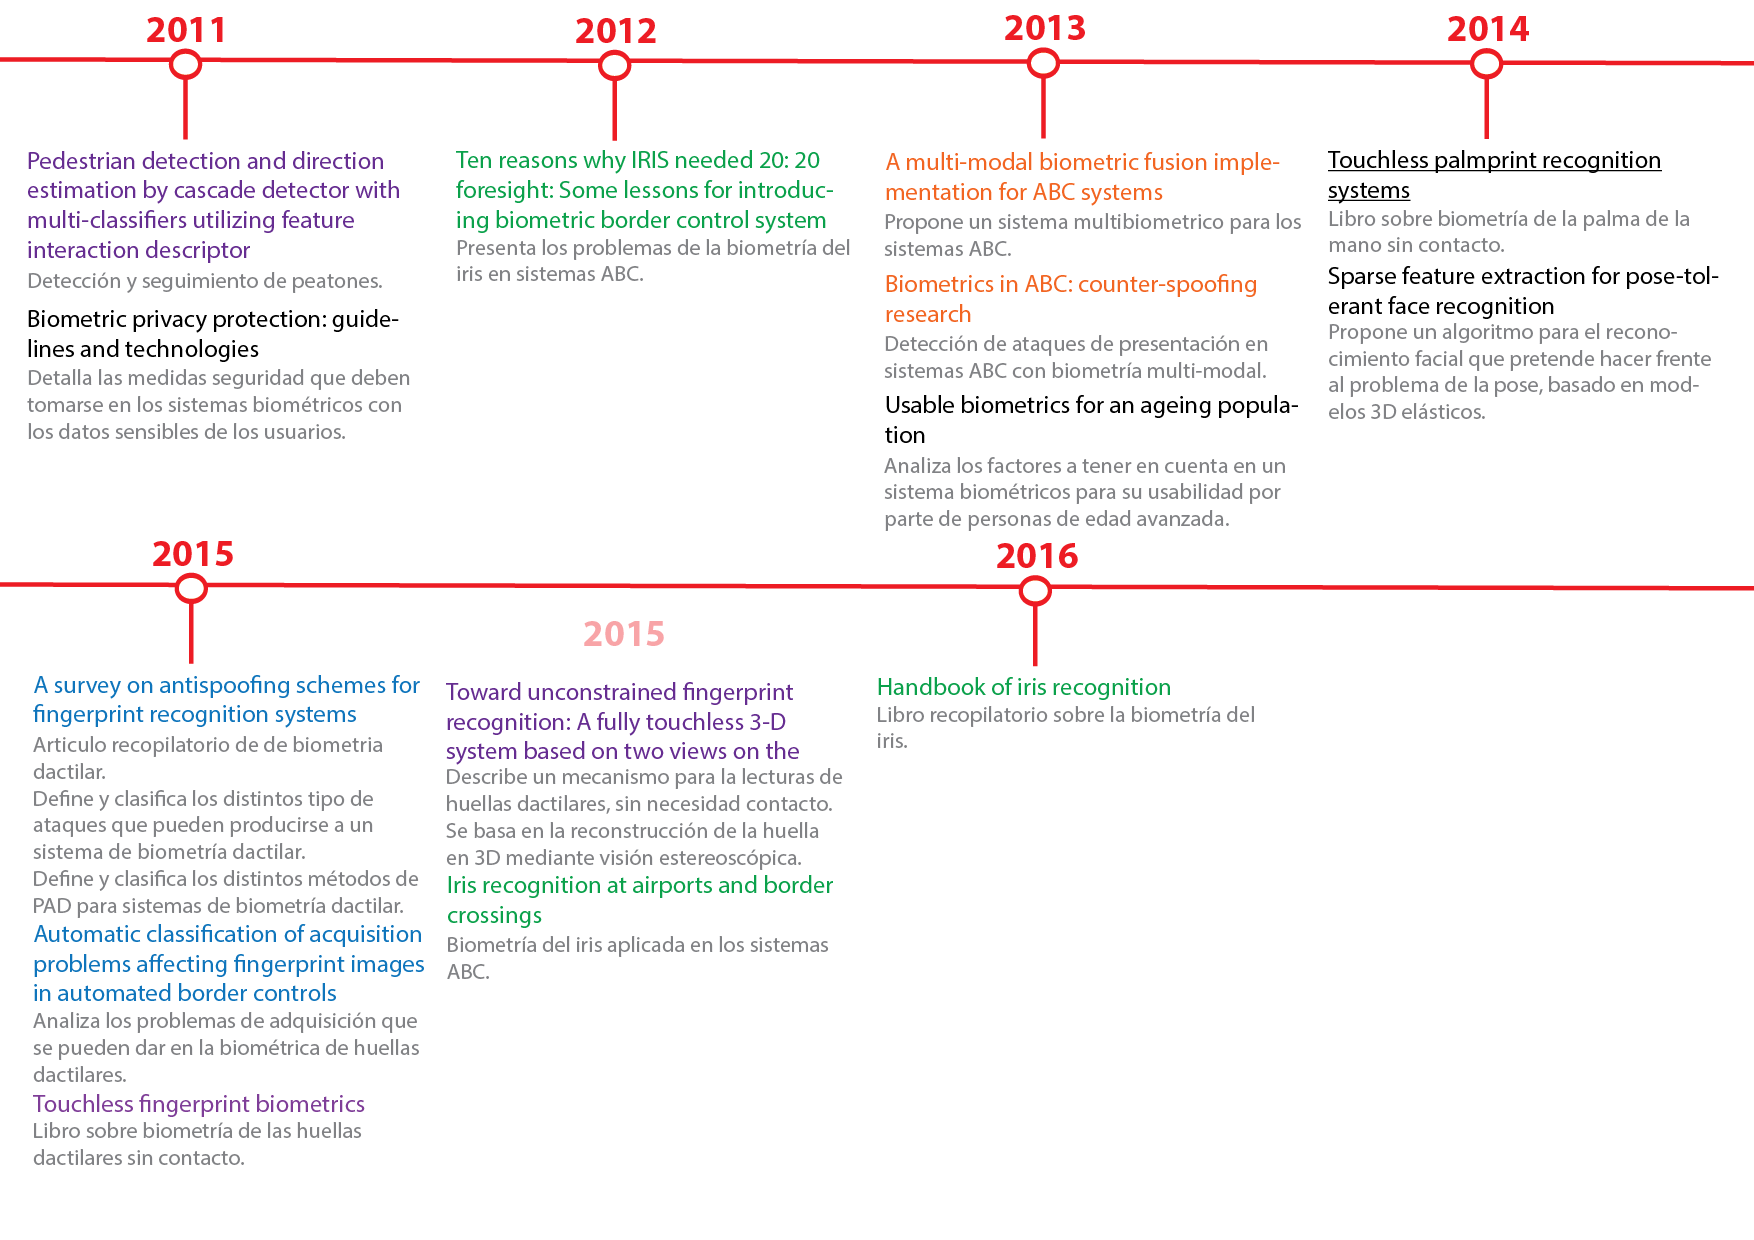
\includegraphics[width=1.4\textwidth]{ch-sistemasABC/images/ch-ImagenesApendices/CRONOLOGIA_BIOMETRIA-02.png}
  \label{fig:01_CRONOLOGIA_BIOMETRIA}
 \end{figure}
\end{landscape}


%IMPLEMENNTACION DE FACENET
$\textbf{2020}$
\cite{SandbergFaceNet}
Implementación de FaceNet


% %%%%%%%%%%%%%%%%%%%%%%%%%%%%%%%%%%%%%%%% BIOMETRIA DACTILAR %%%%%%%%%%%%%%%%%%%%%%%%
% \section{Cronología de publicaciones sobre biometría dactilar}\label{apendix:BiometriaDactilar}

% $\textbf{2005}$

% \cite{gamassi2005fingerprint}
% Verificación dactilar mediante el algoritmo de comparación de minucias.

% \cite{gamassi2005robust}
% Verificación dactilar mediante el algoritmo de comparación de minucias.


% $\textbf{2008}$

% \cite{piuri2008fingerprint}
% Verificación dactilar mediante el algoritmo de comparación de minucias.


% $\textbf{2009}$

% \cite{maltoni2009handbook}
% Libro recopilatorio sobre la biometría dactilar.

% $\textbf{2015}$

% \cite{marasco2015survey}

% Articulo recopilatorio de de \gls{biometria} dactilar.

% Define y clasifica los distintos tipo de ataques que pueden producirse a un sistema de \gls{biometria} dactilar.

% Define y clasifica los distintos métodos de \GLS{PAD} para sistemas de \gls{biometria} dactilar.


% %%%%%%%%%%%%%%%%%%%%%%%%%%%%%%%%%%%%%%%% BIOMETRIA IRIS %%%%%%%%%%%%%%%%%%%%%%%%
% \section{Cronología de publicaciones sobre biometría DEL iris}\label{apendix:BiometriaIris}

% $\textbf{2006}$

% \cite{matey2006iris}
% Presenta un sistema de reconocimiento basado en el iris con adquisición en movimiento \textit{Iris on the Move} (\GLS{IOM})

% $\textbf{2009}$

% \cite{daugman2009iris}
% Algoritmo para la identificación de individuos mediante el iris.

% \cite{chou2009non}
% Propone un algoritmo para reconocimiento del iris con el uso de sensores \GLS{RGB} e \GLS{IR}. Es un algoritmo robusto a los problemas con la pose y que no necesita una vista completamente frontal del iris.

% $\textbf{2012}$

% \cite{palmer2012ten}
% Presenta los problemas de la \gls{biometria} del \gls{iris} en sistemas \GLS{ABC}.

% $\textbf{2015}$

% \cite{daugman2015iris}
% Biometría del iris aplicada en los sistemas \GLS{ABC}


% $\textbf{2016}$

% \cite{bowyer2016handbook}
% Libro recopilatorio sobre la biometría del iris.

% %%%%%%%%%%%%%%%%%%%%%%%%%%%%%%%%%%%%%%%% MULTIBIOMETRIA %%%%%%%%%%%%%%%%%%%%%%%%
% \section{Cronología de publicaciones sobre multibiometría}\label{apendix:Multibiometria}

% $\textbf{2003}$

% \cite{snelick2003multimodal}
% Análisis de sistemas biométricos \gls{multi-modal}

% $\textbf{2004}$

% \cite{jain2004multibiometric}
% Describe las ventajas de usar varios rasgos biométricos en vez de uno sólo.

% \cite{gamassi2004high}
% Define la arquitectura de un sistema multibiometrico con fusión en el subsistema de decisión.

% $\textbf{2006}$

% \cite{ross2006handbook}
% Libro recopilatorio con los distintos métodos de multibiometria.

% \cite{cimato2006personal}
% Describe un sistema multibiometrico con \gls{biometria} facial y \gls{biometria} dactilar.

% El sistema descrito se basa en los \gls{e-passport}, es un sistema similar a los sistemas \GLS{ABC}

% $\textbf{2007}$

% \cite{ISO/Multibiometria}
% Estándar para sistemas biométricos con multibiometria

% \cite{jain2007handbook} 
% libro recopilatorio de \gls{biometria}, con un capitulo deddicado a la \gls{multi-biometria} 

% $\textbf{2008}$

% \cite{cimato2008privacy}
% Propone un sistema multibiométrico que usa \gls{biometria} del iris y \gls{biometria} dactilar.

% $\textbf{2013}$

% \cite{cantarero2013multi}
% Propone un sistema multibiometrico para los sistemas \GLS{ABC}.

% Realiza pruebas con sistemas \GLS{ABC} de un aeropuerto español.

% \cite{wei2013biometrics}  

% Detección de ataques de presentación con biometría multi-modal.


% %%%%%%%%%%%%%%%%%%%%%%%%%%%%%%%%%%%%%%%% BIOMETRIA ON THE FLY %%%%%%%%%%%%%%%%%%%%%%%%
% \section{Cronología de publicaciones sobre biometría OntheFly}\label{apendix:BiometriaOnTheFly}

% $\textbf{2003}$

% \cite{matey2006iris}
% Presenta un sistema con \Gls{biometria} del iris, basado en cámaras de alta resolución, que no requiere que el individuo se detenga frente a la cámara para realizar la adquisición. 


% $\textbf{2011}$
% \cite{goto2011pedestrian}
% Detección y seguimiento de peatones.

% $\textbf{2015}$

% \cite{labati2015touchless}
% Libro recopilatorio de los distintos métodos de \gls{biometria} dactilar sin contacto.

% \cite{labati2015toward}
% Describe un mecanismo para la lecturas de huellas dactilares, sin necesidad contacto. 

% Se basa en la reconstrucción de la huella en $3$D mediante visión estereoscópica.




% %%%%%%%%%%%%%%%%%%%%%%%%%%%%%%%%%%%%%%%% BIOMETRIA GENERAL %%%%%%%%%%%%%%%%%%%%%%%%
% \section{Cronología de publicaciones sobre biometría general}\label{apendix:BiometriaGeneral}

% $\textbf{2003}$

% \cite{snelick2003multimodal}
% Analiza un sistemas biométrica multimodal y presenta distintas técnicas de fusión de la información biométrica.

% $\textbf{2004}$

% \cite{viola2004robust}
% Algoritmo para la detección de caras.

% $\textbf{2009}$

% \cite{li2009encyclopedia}
% Compendio enciclopédico de todos los términos relacionados con la \gls{biometria}.

% \cite{maltoni2009handbook}.
% Libro recopilatorio de biometría dactilar. Estudios, tecnologías y algoritmos.  

% $\textbf{2010}$

% \cite{el2010study}

% \cite{barni2010privacy}
% Analiza los controles y las precauciones necesarias en la \gls{biometria} de huella dactilar para proteger la privacidad de los usuarios.

% $\textbf{2011}$

% \cite{labati2011biometric}
% Detalla las medidas seguridad que deben tomarse en los sistemas biométricos con los datos sensibles de los usuarios.

% $\textbf{2013}$

% \cite{sasse2013usable}
% Analiza los factores a tener en cuenta en un sistema biométricos para su usabilidad por parte de personas de edad avanzada.

% $\textbf{2014}$

% \cite{genovese2014touchless}
% Libro sobre biometría de la palma de la mano sin contacto.

% \cite{abiantun2014sparse}
% Propone un algoritmo para el reconocimiento facial que pretende hacer frente al problema de la pose, basado en modelos 3D elásticos. 


% $\textbf{2015}$

% \cite{labati2015touchless}
% Libro sobre biometría de las huellas dactilares sin contacto. 

% \cite{labati2015toward}
% Reconocimiento de huellas dactilares sin contacto mediante la construcción de un modelo 3D mediante \gls{estereovision}.

% \cite{labati2015automatic}
% Analiza los problemas de adquisición que se pueden dar en la biométrica de huellas dactilares.


% $\textbf{2016}$

% \cite{chen2016unconstrained}
% Reconocimiento facial con redes CNN.


%%%%%% CRONOLOGIA PAD %%%%%%%
\chapter{Cronología de publicaciones sobre PAD}\label{apendix:ApendiceCronologiaPAD}

\begin{landscape}
 \begin{figure}
  \centering
  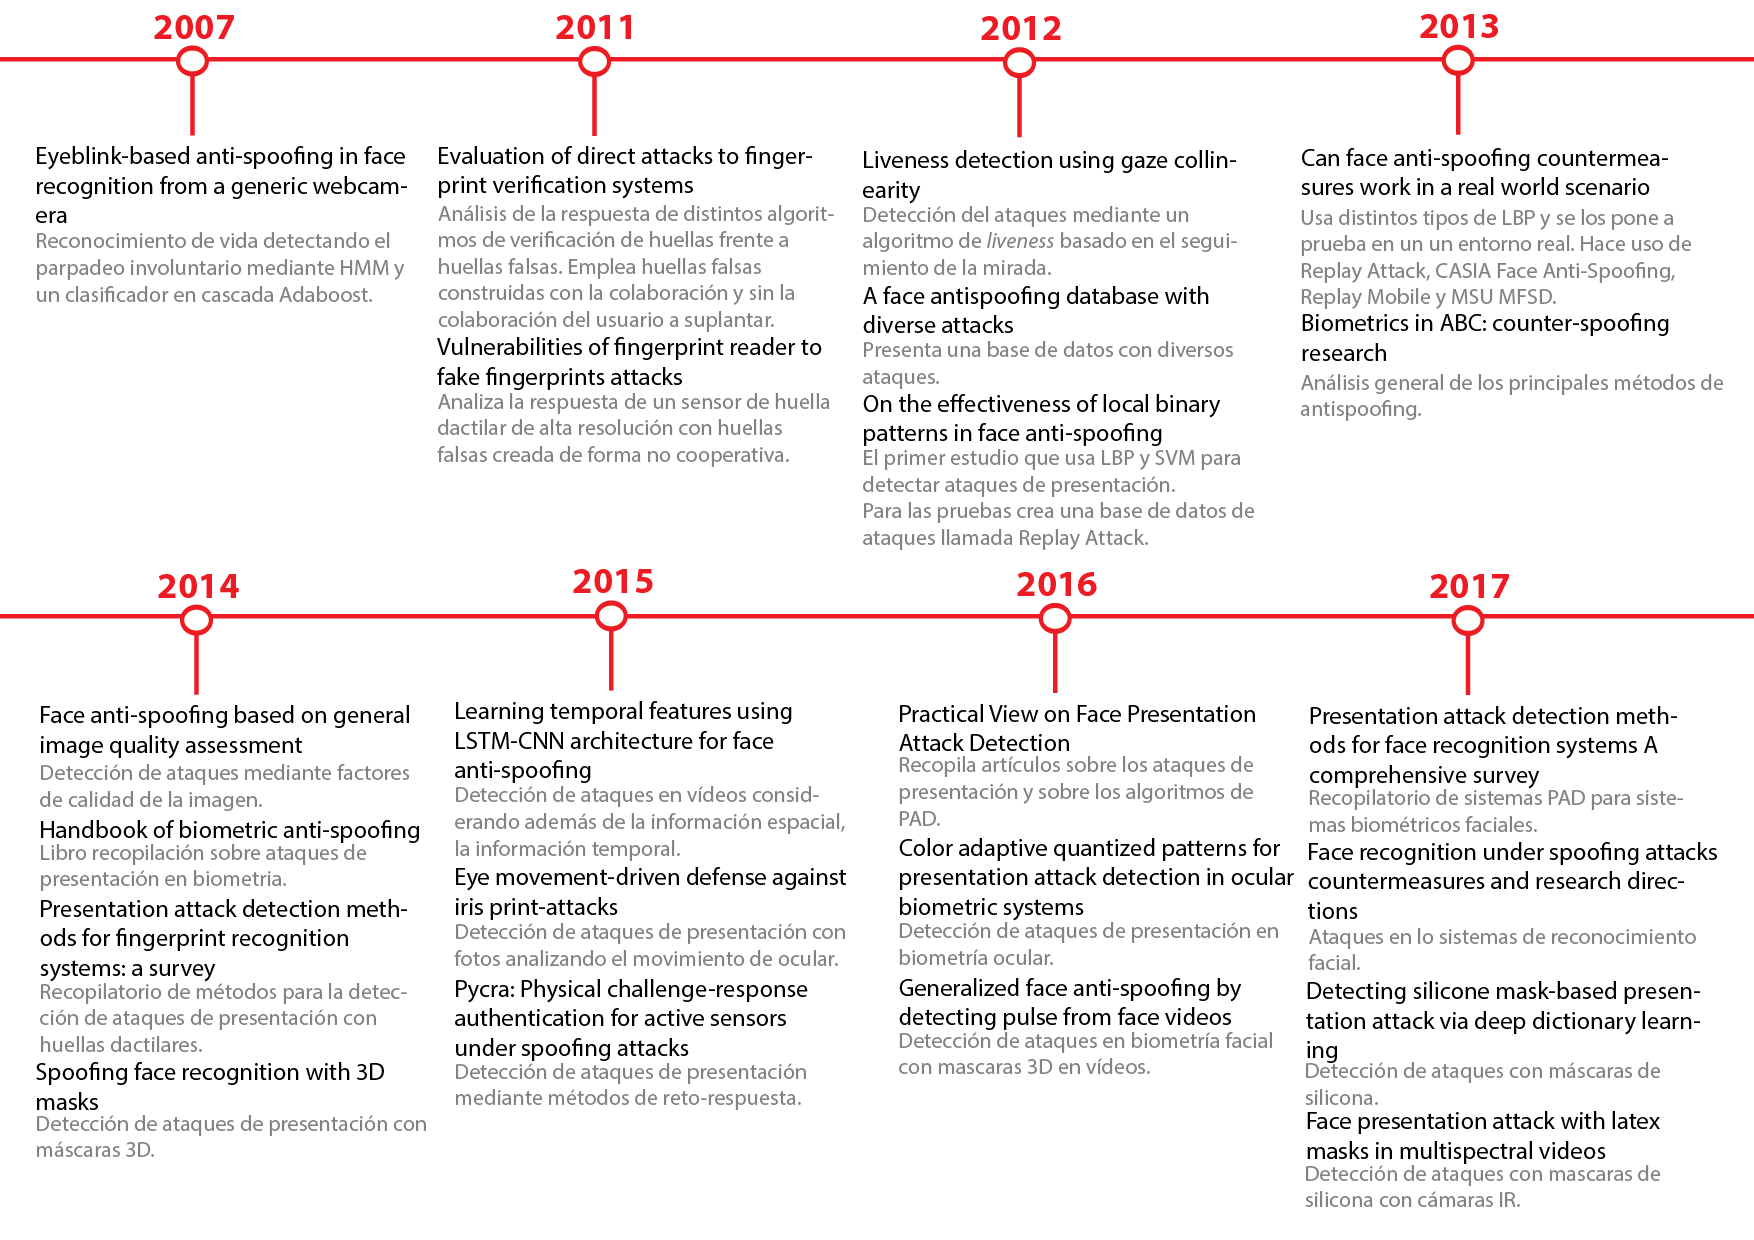
\includegraphics[width=1.4\textwidth]{ch-sistemasABC/images/ch-ImagenesApendices/CRONOLOGIA_PAD-01.png}
  \label{fig:00_CRONOLOGIA_PAD}
 \end{figure}
\end{landscape}

\begin{landscape}
 \begin{figure}
  \centering
  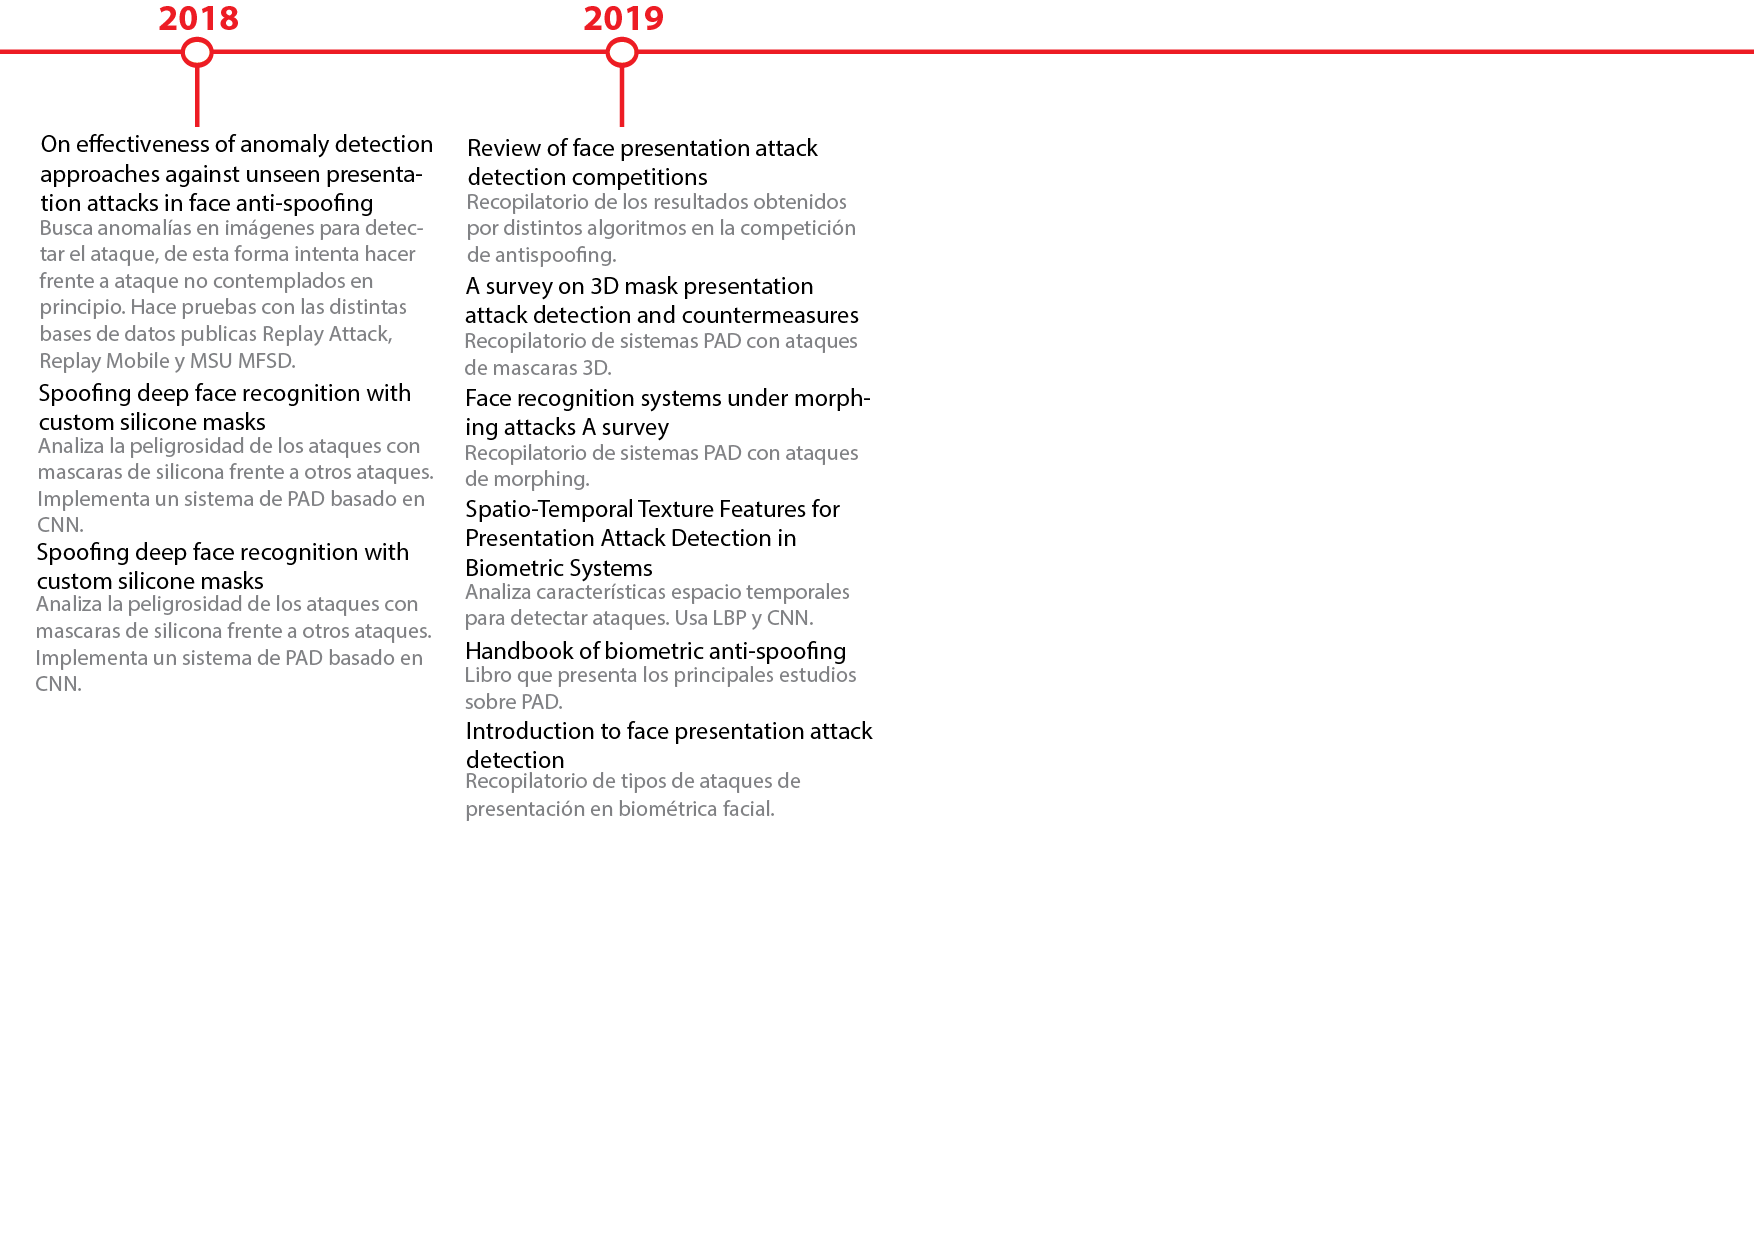
\includegraphics[width=1.4\textwidth]{ch-sistemasABC/images/ch-ImagenesApendices/CRONOLOGIA_PAD-02.png}
  \label{fig:01_CRONOLOGIA_PAD}
 \end{figure}
\end{landscape}


% $\textbf{2007}$

% \cite{pan2007eyeblink}
% Reconocimiento de vida detectando el parpadeo involuntario mediante \gls{HMM} y un clasificador en cascada \textit{Adaboost} 

% $\textbf{2011}$
% \cite{galbally2011evaluation}
% Análisis de la respuesta de distintos algoritmos de verificación de huellas frente a huellas falsas. Emplea huellas falsas construidas con la colaboración y sin la colaboración del usuario a suplantar.

% %ANALIZA LA RESPUESTA DE UN SENSOR DE HUELLA DIGITALES DE ALTA RESOLUCIÓN CON HUELLAS FALSAS CREADAS DE FORMA NO COOPERATIVA 

% \cite{espinoza2011vulnerabilities}
% Analiza la respuesta de un sensor de huella dactilar de alta resolución con huellas falsas creada de forma no cooperativa.

% $\textbf{2012}$

% \cite{ali2012liveness}
% Detección del ataques mediante un algoritmo de \textit{\gls{liveness}} basado en el seguimiento de la mirada.

% \cite{zhang2012face}
% Presenta una base de datos con diversos ataques.

% \cite{chingovska2012effectiveness}
% El primer estudio que usa \gls{LBP} y \gls{SVM} para detectar ataques de presentación.

% Para las pruebas crea una base de datos de ataques llamada \gls{Replay Attack}.

% $\textbf{2013}$

% \cite{de2013can}
% Usa el mismo algoritmo que \cite{chingovska2012effectiveness}, pero prueba distintos tipos de \gls{LBP} y se pone a prueba en un un entorno real.

% Usa la base de datos \gls{Replay Attack} y \gls{CASIA} Face Anti-Spoofing.

% \gls{Replay Attack}, \gls{Replay Mobile} and \gls{MSU MFSD}

% \cite{wei2013biometrics}
% Análisis general de los principales métodos de \gls{antispoofing}.

% $\textbf{2014}$

% \cite{galbally2014face}
% Detección de ataques mediante factores de calidad de la imagen.

% \cite{marcel2014handbook}
% Libro recopilación sobre ataques de presentación en \gls{biometria}.

% \cite{sousedik2014presentation}
% Recopilatorio de métodos para la detección de ataques de presentación con huellas dactilares.

% \cite{erdogmus2014spoofing}
% Detección de ataques de presentación con mascaras $3$D

% $\textbf{2015}$

% \cite{xu2015learning}
% Detección de ataques en vídeos considerando además de la información espacial, la información temporal.

% \cite{rigas2015eye}
% Detección de ataques de presentación con fotos analizando el movimiento de ocular.

% \cite{shoukry2015pycra}
% Detección de ataques de presentación mediante métodos de reto-respuesta.

% $\textbf{2016}$

% \cite{damer2016practical}
% Recopila artículos sobre los ataques de presentación y sobre los algoritmos de \gls{PAD}.

% \cite{raja2016color}
% Detección de ataques de presentación en biometría ocular.

% \cite{li2016generalized}
% Detección de ataques en biometría facial con mascaras 3D en vídeos.

% $\textbf{2017}$

% \cite{ramachandra2017presentation}
% Recopilatorio de sistemas \gls{PAD} para sistemas biométricos faciales. 

% \cite{li2017face}
% Ataques en lo sistemas de reconocimiento facial.

% \cite{manjani2017detecting}
% Detección de ataques con mascaras de silicona.

% \cite{agarwal2017face}
% Detección de ataques con mascaras de silicona con cámaras \GLS{IR}.

% $\textbf{2018}$

% \cite{nikisins2018effectiveness}

% Busca anomalías en imágenes para detectar el ataque, de esta forma intenta hacer frente a ataque no contemplados en principio.

% Hace pruebas con las distintas bases de datos publicas \gls{Replay Attack}, \gls{Replay Mobile} y \gls{MSU MFSD}.

% \cite{bhattacharjee2018spoofing}

% Analiza la peligrosidad de los ataques con mascaras de silicona frente a otros ataques.

% Implementa un sistema de PAD basado en CNN.

% $\textbf{2019}$

% \cite{komulainen2019review}
% Recopilatorio de los resultados obtenidos por distintos algoritmos en la competición de antispoofing.

% \cite{jia2019survey}
% Recopilatorio de sistemas PAD con ataques de mascaras 3D.

% \cite{scherhag2019face}
% Recopilatorio de sistemas PAD con ataques de morphing.

% \cite{pan2019spatio}
% Analiza características espacio temporales para detectar ataques. Usa LBP y CNN.

% \cite{pan2019spatio}
% Libro que presenta los principales estudios sobre PAD.

% \cite{marcel2019handbook}
% Libro recopilación sobre los ataques de presentación en biometría. 

% \cite{hernandez2019introduction}
% Recopilatorio de tipos de ataques de presentación en biométrica facial.


%%%%%%%   CRONOLOGIA MORPHING %%%%%%
\chapter{Cronología de publicaciones sobre morphing}\label{apendix:ApendiceCronologiaMorphing}

\begin{landscape}
 \begin{figure}
  \centering
  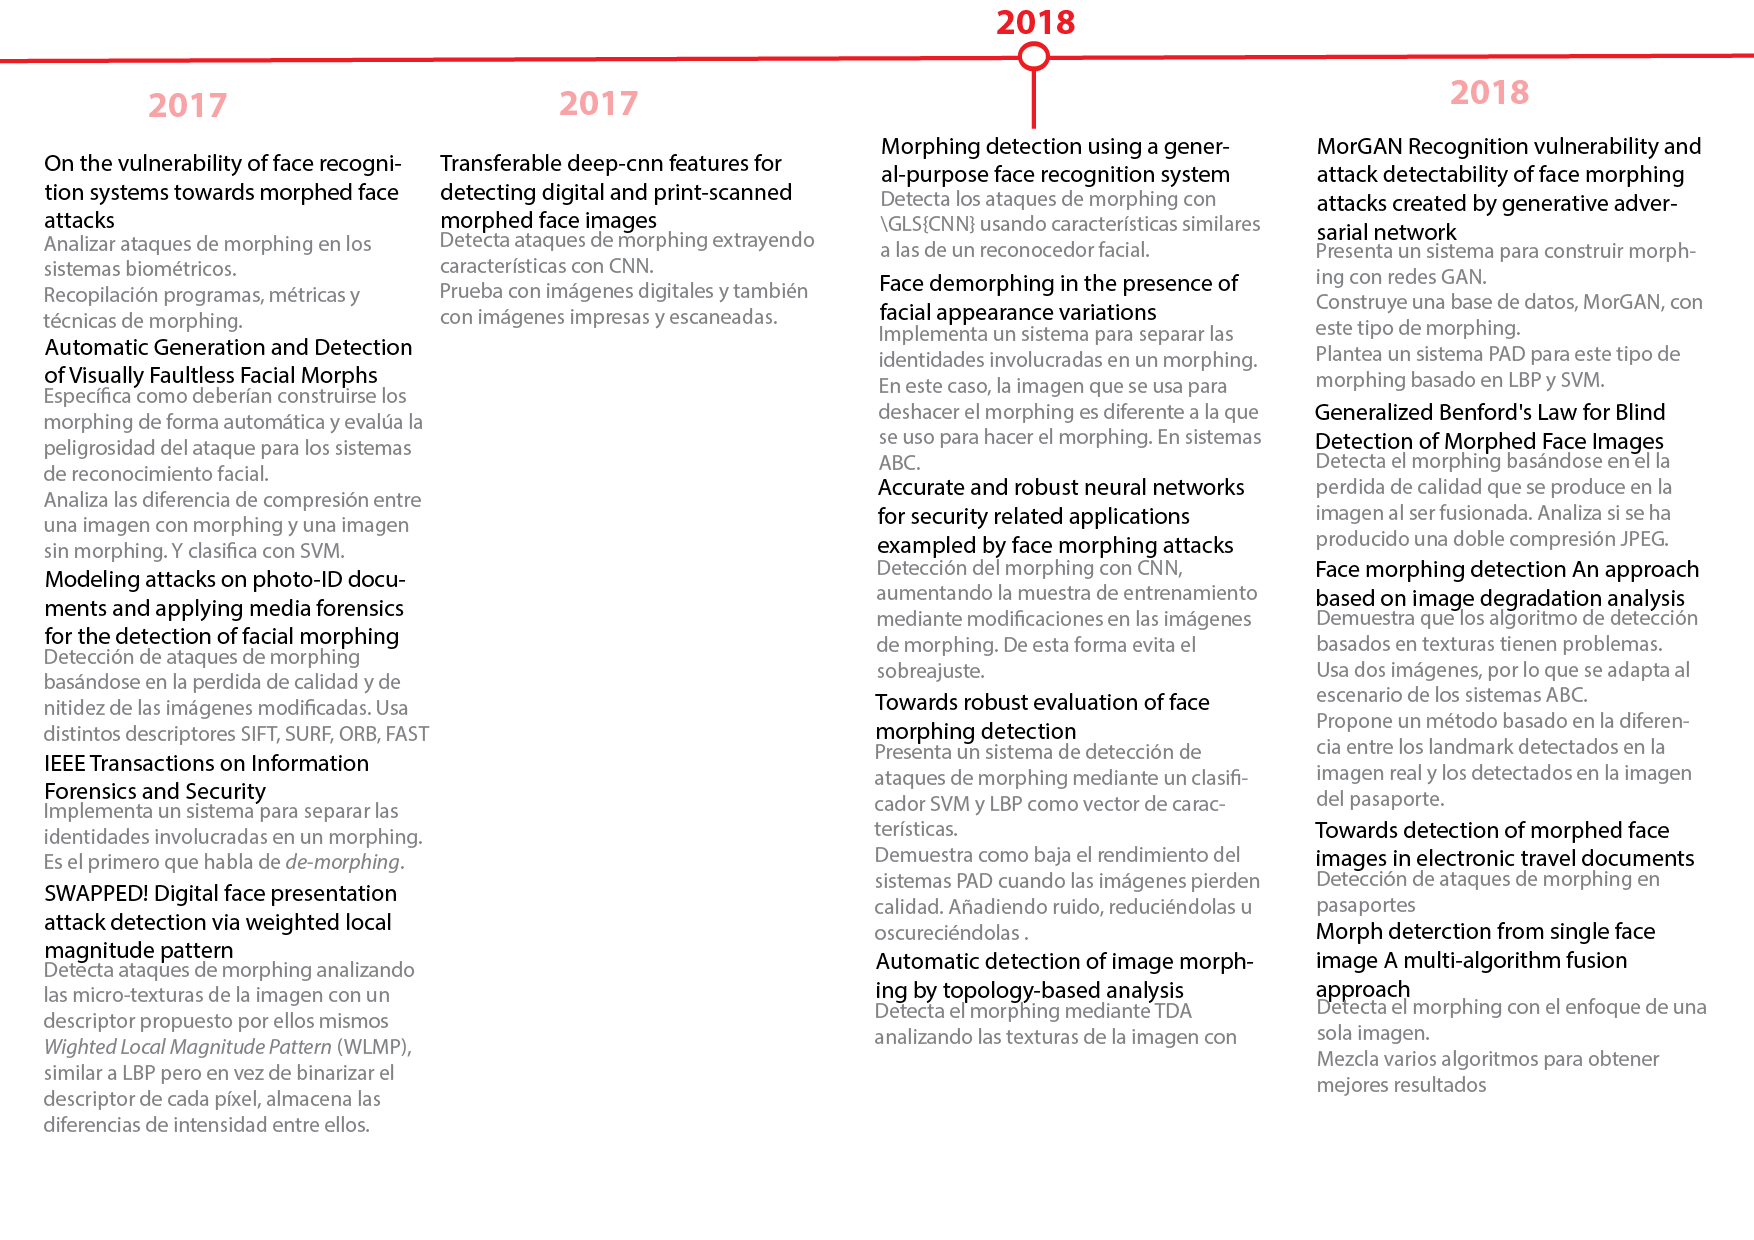
\includegraphics[width=1.4\textwidth]{ch-sistemasABC/images/ch-ImagenesApendices/CRONOLOGIA_MORPHING-02.png}
  \label{fig:01_CRONOLOGIA_MORPHING}
 \end{figure}
\end{landscape}

\begin{landscape}
 \begin{figure}
  \centering
  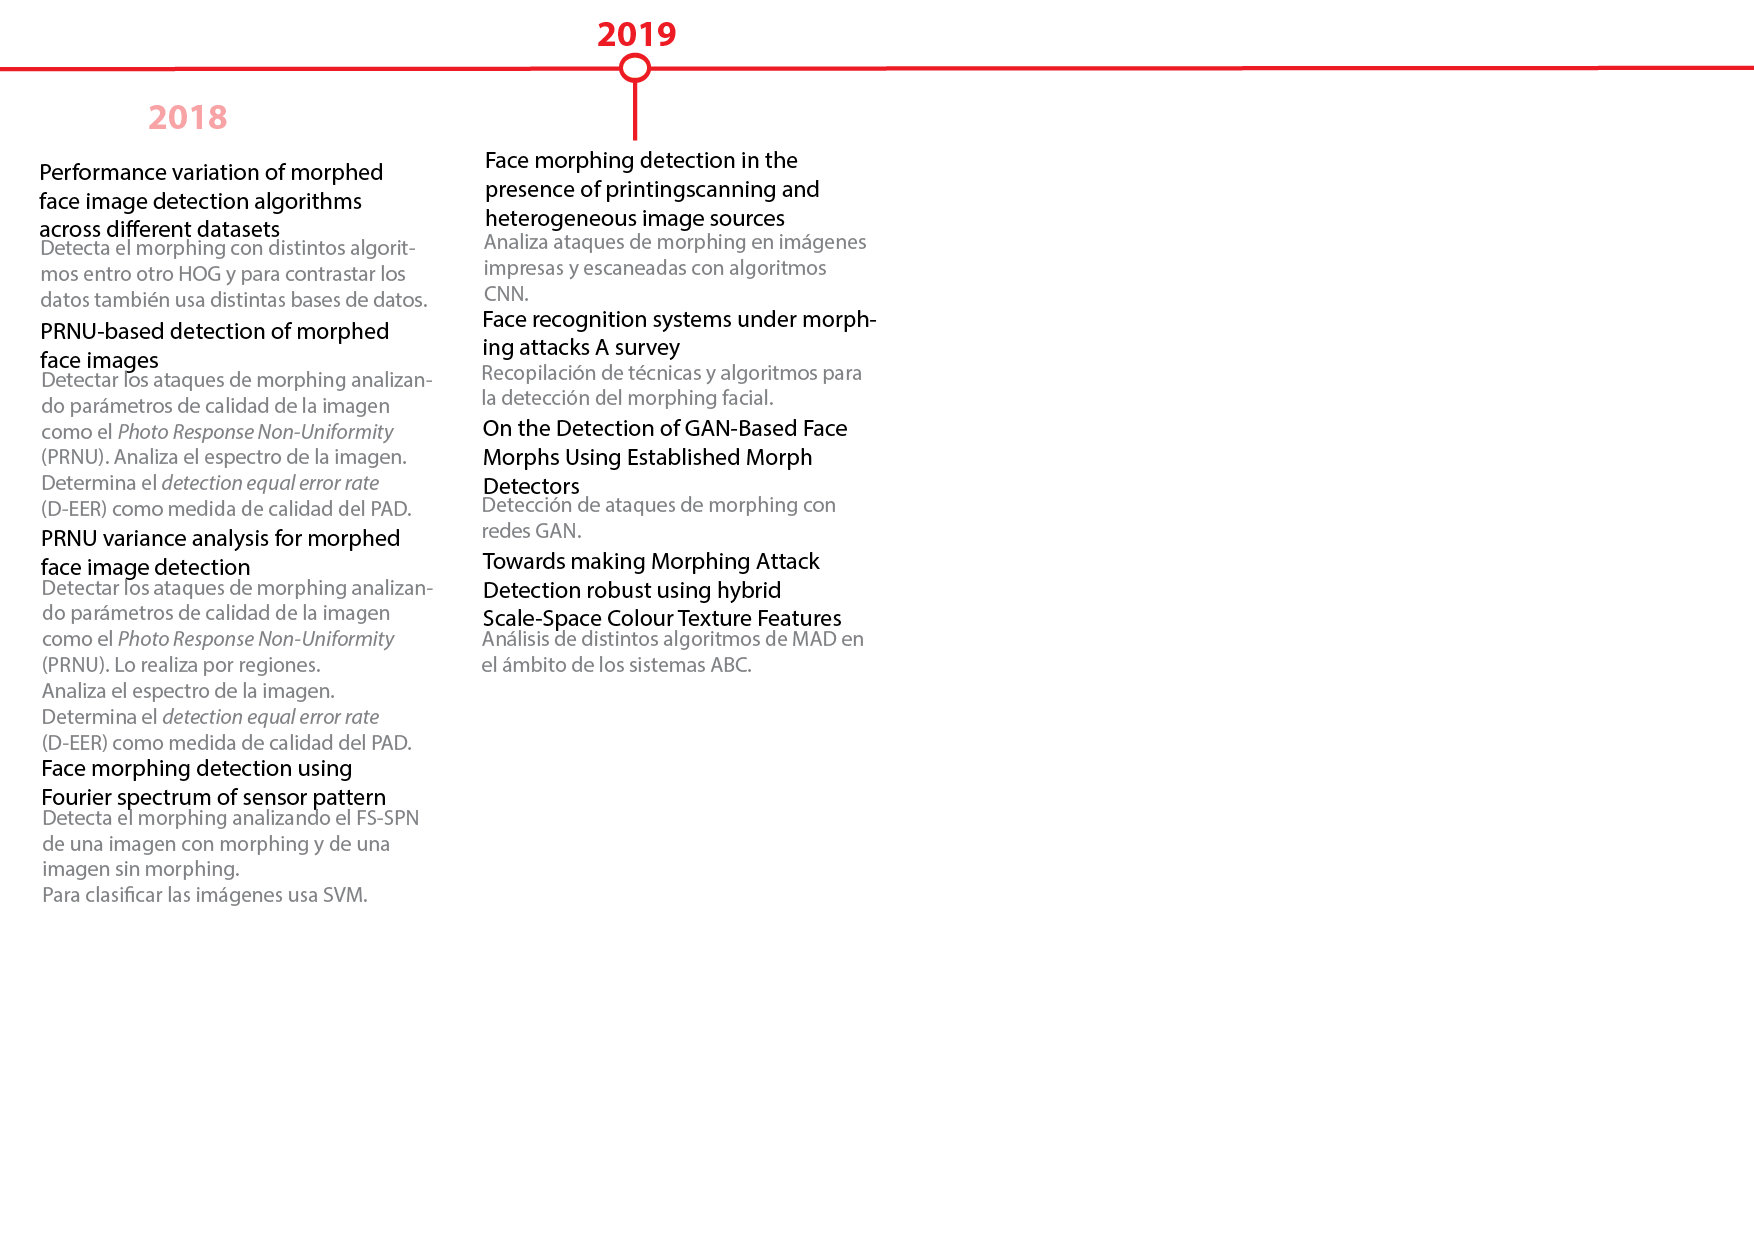
\includegraphics[width=1.4\textwidth]{ch-sistemasABC/images/ch-ImagenesApendices/CRONOLOGIA_MORPHING-03.png}
  \label{fig:02_CRONOLOGIA_MORPHING}
 \end{figure}
\end{landscape}

% NO METIDOS

% $\textbf{2000}$

% \cite{levin2000categorical}


%RECOPILATORIO DE MAD 
% \cite{makrushin2018overview}


% $\textbf{2018}$

% \cite{robertson2018detecting}

% $\textbf{2020}$

%competicion de nist
% \cite{frvtMorphOnLine}
%Competición de algoritmos para la detección de ataques de morphing \GLS(MAD), organizada por \GLS{NIST}.

%DETECCION DE ATAQUES DE MORPHING CON DEMORPHING Y CNN 
%\cite{scherhag2020deep}


% $\textbf{1992}$

% \cite{ucicr1992feature}
% Describe el proceso de morphing para generar efectos visuales que se combinan dos imágenes.

% Es el algoritmo para construir las imágenes del vídeo musical "Black and White" de Michael Jackson.  

% $\textbf{1998}$

% \cite{lee1998polymorph} 
% Describe un algoritmo para la construcción de morphing entre imágenes.

% \cite{wolberg1998image}
% Recopilatorio de algoritmos de construcción de imágenes morphing

% $\textbf{2011}$

% \cite{wu2011face}
% Descripción detallada de la construcción del morphing mediante triangulación, de las posibles mejoras y de la problemática.

% $\textbf{2013}$

% \cite{lokhande2013morphing}
% Recopilatorio de técnicas para la construcción de morphing. Incluye la construcción mediante \textit{Delaunay-Voronoi triangulation} (\GLS{DVT}).

% $\textbf{2014}$ 

% \cite{ferrara2014magic}
% Definición del problema del morphing como ataque de presentación.

% $\textbf{2016}$

% \cite{ferrara2016effects}
% Detección de modificaciones en la imagen desde el espectro de frecuencia de la imagen. 

% \cite{raghavendra2016Detecting}
% Detección de ataques de morphing con distintos descriptores: \GLS{LBP}, \GLS{BSIF} y con un clasificador \GLS{SVM}. 

% \cite{goodfellow2016deep}
% Detección de los ataques de morphing con distintas arquitecturas de red convolución (AlexNet, GoogleLeNet y VGG19), entrenadas desde cero o pre-entrenadas.  

% $\textbf{2017}$

% \cite{ferrara2016feasibility}
% \Gls{morphing} con huellas dactilares.

% \cite{rathgeb2017feasibility}
% \Gls{morphing} con imágenes del iris.

% \cite{raghavendra2017face}
% Estudia la detección del morphing con \gls{LBP} y \gls{SVM}.

% Compara los resultados de una fusión calculando la media entre dos imágenes faciales y el morphing completo.

% Prueba con imágenes impresas y escaneadas.

% \cite{asaad2017topological}
% Estudia la detección del morphing en imágenes basándose su \textit{Topological Data Analysis} (\GLS{TDA}).

% Analiza la textura de las imágenes morphing con \GLS{LBP}.

% \cite{neubert2017face}
% Busca detectar el morphing con descriptores espaciales como \GLS{SIFT} o \GLS{SURF}. Y se centra en analizar como afecta la compresión \GLS{JPEG} en la detección.

% \cite{hildebrandt2017benchmarking}
% Evalúa la detección de morphing, cuando se le aplican distintas mejoras al proceso de construcción del morphing.

% \cite{scherhag2017biometric}
% Analizar ataques de morphing en los sistemas biométricos.

% Proponen unas métricas: \GLS{MMPMR} \GLS{RMMR} para evaluar el impacto de los ataques de morphing en los sistemas de reconocimiento facial. 

% Recomendaciones a tener en cuenta para la construcción de morphing.

% Propone el uso de un índice para medir la calidad de las imágenes \GLS{BRISQUE}\cite{mittal2011blind}. 

% AtaquesMorphingASistemasBiometricos

% \cite{scherhag2017vulnerability}
% Analizar ataques de morphing en los sistemas biométricos.

% Recopilación programas, métricas y técnicas de morphing.  

% \cite{makrushin2017automatic}
% Específica como deberían construirse los morphing de forma automática y evalúa la peligrosidad del ataque para los sistemas de reconocimiento facial.

% Analiza las diferencia de compresión entre una imagen con morphing y una imagen sin morphing. Y clasifica con SVM.

% \cite{kraetzer2017modeling}
% Detección de ataques de morphing basándose en la perdida de calidad y de nitidez de las imágenes modificadas. Usa distintos descriptores \gls{SIFT}, \gls{SURF}, \gls{ORB},\gls{FAST} o \gls{AGAST}.

% \cite{ferrara2017face}
% Implementa un sistema para separar las identidades involucradas en un morphing.

% Es el primero que habla de \textit{\gls{de-morphing}}.

% \cite{agarwal2017swapped}
% Detecta ataques de morphing analizando las micro-texturas de la imagen con un descriptor propuesto por ellos mismos \textit{Wighted Local Magnitude Pattern} (\gls{WLMP}), similar a \GLS{LBP} pero en vez de binarizar el descriptor de cada píxel, almacena las diferencias de intensidad entre ellos.

% \cite{raghavendra2017transferable}
% Detecta ataques de morphing extrayendo características con \GLS{CNN}.

% Prueba con imágenes digitales y también con imágenes impresas y escaneadas.


% $\textbf{2018}$

% \cite{wandzik2018morphing}
% Detecta los ataques de morphing con \GLS{CNN} usando características similares a las de un reconocedor facial.

% \cite{ferrara2018face}
% Implementa un sistema para separar las identidades involucradas en un morphing. 
% En este caso, la imagen que se usa para deshacer el morphing es diferente a la que se uso para hacer el morphing. 

% En sistemas \GLS{ABC}

% \cite{seibold2018accurate}
% Detección del morphing con \gls{CNN}, aumentando la muestra de entrenamiento mediante modificaciones en las imágenes de morphing. De esta forma evita el sobreajuste. 

% \cite{spreeuwers2018towards}
% Presenta un sistema de detección de ataques de morphing mediante un clasificador \gls{SVM} y \gls{LBP} como vector de características. 

% Demuestra como baja el rendimiento del sistemas \gls{PAD} cuando las imágenes pierden calidad. Añadiendo ruido, reduciéndolas u oscureciéndolas    

% \cite{seibold2018reflection}
% Detección de los ataques de morphing analizando la reflexión y la luminosidad de las imágenes.

% \cite{jassim2018automatic}
% Detecta el morphing mediante \gls{TDA} analizando las texturas de la imagen con LBP.

% \cite{damer2018morgan}
% Presenta un sistema para construir morphing con redes \gls{GAN}.

% Construye una base de datos, \gls{MorGAN}, con este tipo de morphing.

% Plantea un sistema \gls{PAD} para este tipo de morphing basado en LBP y SVM.

% \cite{makrushin2018generalized}
% Detecta el morphing basándose en el la perdida de calidad que se produce en la imagen al ser fusionada. Analiza si se ha producido una doble compresión \gls{JPEG}.

% \cite{neubert2017face}
% Demuestra que los algoritmo de detección basados en texturas tienen problemas.

% Usa dos imágenes, por lo que se adapta al escenario de los sistemas ABC.

% Propone un método basado en la diferencia entre los \gls{landmark} detectados en la imagen real y los detectados en la imagen del pasaporte.

% \cite{scherhag2018towards}
% Detección de ataques de morphing en pasaportes

% \cite{scherhag2018morph}
% Detecta el morphing con el enfoque de una sola imagen.

% Mezcla varios algoritmos para obtener mejores resultados.

% \cite{scherhag2018performance}
% Detecta el morphing con distintos algoritmos entro otro \gls{HOG} y para contrastar los datos también usa distintas bases de datos.

% \cite{debiasi2018prnu}
% Detectar los ataques de morphing analizando parámetros de calidad de la imagen como el \textit{Photo Response Non-Uniformity} (\gls{PRNU})

% Analiza el espectro de la imagen.

% Determina el \textit{detection equal error rate} (\gls{D-EER}) como medida de calidad del \GLS{PAD}.

% \cite{debiasi2018prnuvar}
% Detectar los ataques de morphing analizando parámetros de calidad de la imagen como el \textit{Photo Response Non-Uniformity} (\gls{PRNU}). A diferencia de \cite{debiasi2018prnu}, lo realiza por regiones.

% Analiza el espectro de la imagen.

% Determina el \textit{detection equal error rate} (\gls{D-EER}) como medida de calidad del \GLS{PAD}.

% %DETECTA EL MORPHING CON SVM APOYANDOSE EN FS-SPN (FURIER ESPECTRO)
% \cite{zhang2018face}
% Detecta el morphing analizando el \gls{FS-SPN} de una imagen con morphing y de una imagen sin morphing. 

% Para clasificar las imágenes usa \gls{SVM}.

% \textbf{2019}

% \cite{ferrara2019face}
% Analiza ataques de morphing en imágenes impresas y escaneadas con algoritmos \GLS{CNN}. 

% \cite{scherhag2019face}
% Recopilación de técnicas y algoritmos para la detección del morphing facial.

% \cite{debiasi2019detection}
% Detección de ataques de morphing con redes \GLS{GAN}.

% \cite{ramachandra2019towards}
% Análisis de distintos algoritmos de \gls{MAD} en el ámbito de los sistemas \GLS{ABC}.
